%% latex_185_moulds_g.tex
%%
%% The following file is a skeleton file that demonstrates how to implement the IEEEtran.cls class 
%% file in LaTeX. This file is intended for the CMPE185 Technical Writing for Engineers Course in 
%% which the students must write a tutorial aimed towards novice LaTeX users in the LaTex environment.
%%
%% This file is heavily adapted from Michael Shell's bare_adv.tex file made available at 
%% http://www.ieee.org/conferences_events/conferences/publishing/templates.html
%%
%% You will need to rename this file with your information in the following format:
%% latex_185_last name_ first initial.tex
%% ---------------------------------------------------------------------------------------------------

% \documentclass{} precedes the preamble and is typically the first command in any .tex document. Every .tex document should include this command as it defines what kind of document you intend on creating. Modifiers in square brackets [] can be added in between the text ''documentclass'' and the curly brackets {} to modify font size, templates, etc. 

\documentclass[12pt,journal,compsoc]{IEEEtran}

%-----PACKAGES-------------------------------------------------------------------------------------

% Packages include extra commands that allow for additional formatting, ranging from Graphics, Math, to Alignment. The command to include packages will always look similar to \usepackage{} where the package name is within the curly brackets {}. Packages are defined in the preamble, i.e., between the \documentclass{} and \begin{document} commands.

% The following link takes you to a list of additional packages that may not be listed here. http://en.wikibooks.org/wiki/LaTeX/Package_Reference

% TO INCLUDE PACKAGES: 
% - Open the file ''latex_sample_packages.tex'' from the .zip folder.
% - From this file, COPY the code for the package you want to include and PASTE into your own .tex file.
% - Uncomment the package you want to include and load, i.e., remove the ''%'' in front of the \usepackage{package_name}.
 

% Copy package text here:

\usepackage{graphicx}
% This is an example of how a \usepackage{} command should be included. You will need to include more packages to complete this assignment.




%----- The DOCUMENT Environment-------------------------------------------------------------------

% The \begin{document} and \end{document} commands establish the environment for the text of the document. The \begin{} and \end{} commands are used repeatedly in LaTeX to show where an environment begins and ends. The \end{document} command will be the last line of this .tex file.

\begin{document}

% The following commands are self explanatory. Insert your title, author and date into each command's curly bracket. You can include the abstract, paper header and paper footer information in this section then conclude the section with the command \maketitle (shown as the last line at the end of this section).

\title{Basic \LaTeX{}}
\author{Jason Bonilla\\
		CSE185 \\
		University of California, Santa Cruz \\
		\date{10-22-2020}
		}
% The double backslash \\ is used here to enter a ''Carriage Return'', or a line break. Note that the tilde ~ in between my name used as a ''Nonbreaking Space''. LaTeX will not break a structure at a ~ so this keeps an author's name from being broken across two lines. Also note that I included my name as an example so make sure to only insert your name in this command.

\date{}		% leaving the brackets empty omits the date
% To input the current date, you can type: \date{\today}

% The paper headers
\markboth{\LaTeX\ IEEE Template Tutorial}%
{Moulds \MakeLowercase{\textit{et al.}}: CMPE185}
% The only time the second header will appear is for the odd numbered pages
% after the title page when using the twoside option.
% 
% *** Note that you probably will NOT want to include the author's ***
% *** name in the headers of peer review papers.                   ***
% You can use \ifCLASSOPTIONpeerreview for conditional compilation here if
% you desire.

% The publisher's ID mark at the bottom of the page is less important with
% Computer Society journal papers as those publications place the marks
% outside of the main text columns and, therefore, unlike regular IEEE
% journals, the available text space is not reduced by their presence.
% If you want to put a publisher's ID mark on the page you can do it like
% this:
\IEEEpubid{0000--0000/00\$00.00~\copyright~2007 IEEE}
% or like this to get the Computer Society new two part style.
%\IEEEpubid{\makebox[\columnwidth]{\hfill 0000--0000/00/\$00.00~\copyright~2007 IEEE}%
%\hspace{\columnsep}\makebox[\columnwidth]{Published by the IEEE Computer Society\hfill}}
% Remember, if you use this you must call \IEEEpubidadjcol in the second
% column for its text to clear the IEEEpubid mark (Computer Society jorunal
% papers don't need this extra clearance.)


% use for special paper notices
%\IEEEspecialpapernotice{(Invited Paper)}

% for Computer Society papers, we must declare the abstract and index terms
% PRIOR to the title within the \IEEEcompsoctitleabstractindextext IEEEtran
% command as these need to go into the title area created by \maketitle.
\IEEEcompsoctitleabstractindextext{%
\begin{abstract}
%\boldmath
The abstract goes here.
\end{abstract}
% IEEEtran.cls defaults to using nonbold math in the Abstract.
% This preserves the distinction between vectors and scalars. However,
% if the journal you are submitting to favors bold math in the abstract,
% then you can use LaTeX's standard command \boldmath at the very start
% of the abstract to achieve this. Many IEEE journals frown on math
% in the abstract anyway. In particular, the Computer Society does
% not want either math or citations to appear in the abstract.

% Note that keywords are not normally used for peerreview papers.
\begin{IEEEkeywords}
CMPE185, \LaTeX\ Tutorial, IEEEtran, journal, \LaTeX, paper, template.
\end{IEEEkeywords}}

\maketitle

%----- The SECTION Environment -------------------------------------------------------------------

% To create a section, simply type the command \section{} with the name of your section name inserted into the curly brackets {}. The section's body text follows underneath the \section{} command. 

\section{Introduction}
% Computer Society journal papers do something a tad strange with the very
% first section heading (almost always called "Introduction"). They place it
% ABOVE the main text! IEEEtran.cls currently does not do this for you.
% However, You can achieve this effect by making LaTeX jump through some
% hoops via something like:
%
%\ifCLASSOPTIONcompsoc
%  \noindent\raisebox{2\baselineskip}[0pt][0pt]%
%  {\parbox{\columnwidth}{\section{Introduction}\label{sec:introduction}%
%  \global\everypar=\everypar}}%
%  \vspace{-1\baselineskip}\vspace{-\parskip}\par
%\else
%  \section{Introduction}\label{sec:introduction}\par
%\fi
%
% Admittedly, this is a hack and may well be fragile, but seems to do the
% trick for me. Note the need to keep any \label that may be used right
% after \section in the above as the hack puts \section within a raised box.



% The very first letter is a 2 line initial drop letter followed
% by the rest of the first word in caps (small caps for compsoc).
% 
% form to use if the first word consists of a single letter:
% \IEEEPARstart{A}{demo} file is ....
% 
% form to use if you need the single drop letter followed by
% normal text (unknown if ever used by IEEE):
% \IEEEPARstart{A}{}demo file is ....
% 
% Some journals put the first two words in caps:
% \IEEEPARstart{T}{his demo} file is ....
% 
% Here we have the typical use of a "T" for an initial drop letter
% and "HIS" in caps to complete the first word.

\IEEEPARstart{T}{his} is a tutorial on the basics of \LaTeX\ . \LaTeX\ is a free typesetting language created by Leslie Lamport in order to make it easier to produce general-purpose books and articles within TeX. Because \LaTeX\ is an extension to the TeX typesetting system, \LaTeX\ is popular with scientists and engineers.
% You must have at least 2 lines in the paragraph with the drop letter
% (should never be an issue)
 

% Creating a subsection is similar to creating a section and is used with the command \subsection{}.



\section{Creating a .tex file}
All Latex files are in the .tex format. Creating an account in Overleaf and opening a new file is a very simple way to create a .tex file. Thankfully Professor Moulds was generous enough to give us a zip file containing a .tex file already.

\subsection{Environments}
In order to begin a document you must start with command \textbackslash{begin\{\}} and end with \textbackslash{end\{\}} . There are several other keywords in \LaTeX\ that follow the \textbackslash{*keyword*\{\}} format. Including \textbackslash{begin\{\}} and \textbackslash{end\{\}} is very important in order to avoid errors during the compiling process.

\subsection{Reserved Characters}
Reserved characters or special characters are characters that have a specific function in \LaTeX\  .Here are a few of the most popular ones \begin{center}
  \# \$ \% \& \{ \} \_ \~{} \^{} \textbackslash \\
\end{center}
The \% is a very useful character, it comments out lines in the code that do not show up when the document is compiled. \textbackslash is used before every function or special character. \textbackslash \textbackslash  creates  a line  break like this. Tilde (~) is used in LaTeX code to produce non-breakable space. Because these characters are reserved, they will throw an error if you are to simply type them out in your \LaTeX\ document. You must add a \textbackslash in front of each reserved character in order for them to be displayed normally like so: \textbackslash \#  \textbackslash \$ \textbackslash \& \textbackslash \_ \\  For a more detailed explanation of each character and symbol I would recommend checking out
\begin{center}


\textbf{Special Characters and Symbols}
\text{https://www.dickimaw-books.com/latex/novices/html/symbols.html} 
\end{center}


\subsection{Preamble}
The preamble is the first section of an input file, before the text of the document itself, in which you tell the \LaTeX\ the type of document, and other information \LaTeX\ will need to format the document correctly. It contains packages, document class, title, author, and the date. Packages have extra commands that let you customize your document and add extras to it. In order to add a package, you need to type \textbackslash{usepackage\{*your package name*\}}. A simple google search will allow you to find any package you are looking for. It is necessary to include what type of document you are using. \LaTeX\ supports reports, articles, slides, and many more. You can specify this by  using the \textbackslash{documentclass\{*document type*\}}. All you have to do in order to get started working on your document is put all your information in between \textbackslash{documentclass\{*document type*\}} and \textbackslash{end\{*document type*\}}. It is important to note, that you can specify font sizes in two levels, the first being with the documentclass command like so \textbackslash{documentclass[12pt]\{report\} } and the second being inline to a smaller portion of text instead of the entire document. Here is a link that goes into more detail:
\begin{center}
    https://texblog.org/2012/08/29/changing-the-font-size-in-latex/
\end{center}

\subsection{Title and Heading Information}
In order to make a title in \LaTeX\ , you must start with \textbackslash{title\{\}} and end with \textbackslash{maketitle}. In between those two you can specify many things including who the author is using \textbackslash{author\{\}} and the date using \textbackslash{date\{\}}. Below I will show an example of how I made the exact title I used for this document below.

\begin{center}
\textbackslash{title}\{Basic\textbackslash{LaTeX\{\}} \} \\
 \textbackslash{author} \{ Jason Bonilla \textbackslash \textbackslash \\
          CSE185, \textbackslash \textbackslash \\
          University of California, Santa Cruz \textbackslash \textbackslash \\
           \textbackslash{date\{{10-22-2020}}
       \} \}\textbackslash \textbackslash  \\
 \textbackslash{maketitle}\\
 \end{center}

\section{Sections}
\LaTeX\ can organize, number, and index chapters and sections of document. There are up to 7 levels of depth for defining sections depending on the document class. In order to create this paragraph I used \textbackslash{section\{section\}}. If you would wish to not include a number with each section you would simply put a * like so \textbackslash{section*\{section\}}.

\begin{center}
    \textbackslash{part\{part\}} \\
    \textbackslash{chapter\{chapter\}} \\
    \textbackslash{section\{section\}} \\
    \textbackslash{subsection\{subsection\}} \\
    \textbackslash{subsubsection\{subsubsection\}}
    \textbackslash{paragraph\{paragraph\}}
    \textbackslash{subparagraph\{subparagraph\}}

\end{center}

\subsection{Subsections}
Subsections are very similar to sections, in the way that they are used to organize a document. But a subsection, is typically a more specific part of the very general section that it belongs to. You can use a subsection by using \textbackslash{subsection\{subsection\}}

\section{Body Text: Paragraphs and Content}
Even though the default formatting in \LaTeX\ is fine, sometimes we need to change some elements. In order to format a paragraph in the center you can use \textbackslash{begin\{center\}}  *insert content here* \textbackslash{end\{center\}}

\begin{center}
    This is an example of having a centered stand alone paragraph.
\end{center}
To start a new paragraph in \LaTeX\, you can \textbackslash \textbackslash or use the command \textbackslash{par} after the last sentence in the paragraph that you wish to end. This will however indent both paragraphs. Below is an example of how to use the command: \\

What you doin' in the club on a Thursday?
She say she only here for her girl birthday. \par
They ordered champagne but still look thirsty.
Rock Forever 21 but just turned thirty.


\section{Tables}
\LaTeX\ already has built-in support to typeset tables.
For beginners it may be a bit confusing, since \LaTeX\
provides two environments: tabular and table. To
typeset material in rows and columns, tabular is
needed, while the table environment is a container
for floating material similar to figure, into which a
tabular environment may be included. Here is an example of a tabular without the use of a table container 

\begin{center}
  \begin{tabular}{ | l | c | r | }
    \hline
    1 & 2 & 3 \\ \hline
    4 & 5 & 6 \\ \hline
    7 & 8 & 9 \\ 
    \hline
  \end{tabular}
\end{center}

Here is an example of a tabular within a table container

\begin{table}[h]\footnotesize
  \caption{Performance at peak F-measure}
  \begin{center}
  \begin{tabular}{ | l | c | r | }
    \hline
    1 & 2 & 3 \\ \hline
    4 & 5 & 6 \\ \hline
    7 & 8 & 9 \\ 
    \hline
  \end{tabular}
\end{center}
\end{table} \\

As you see, table is the outer container, creating a floating table object with a title and a caption, whereas tabular is the inner container, creating the actual grid of table cells. Tables offer more flexibility than a tabular, but tabulars are  favored for their simplicity. Tables and tabulars could not be made possible without the following symbols.

\begin{center}
    
    \begin{table}[h]
  \caption{Symbols}
  \begin{center}
  \begin{tabular}{ | l | r | }
    \hline
    l & left-justified column  \\ \hline
    c & centered column  \\ \hline
    r & right-justified column  \\ \hline
    \textbar & vertical line  \\ \hline
    \textbar\ \textbar\ & double vertical line  \\ \hline
    \textbackslash{hline} & horizontal line  \\ \hline
    \textbackslash \textbackslash\ & new line  \\ \hline
  \end{tabular}
\end{center}
\end{table}
\end{center}

Here is the code used to make the table above using [h] for positioning ,l, c, r, \textbackslash{hline}, \textbackslash \textbackslash, and \textbar. Alternatively you can use [t],[b],[p],[H], or [!] for different positions.

\begin{center}
    
    \textbackslash{begin\{table\}}[h] \textbackslash{footnotesize} \\
    \textbackslash{caption\{Performance at peak F-measure\}} \\
    \textbackslash{begin\{center\}} \\
    \textbackslash{begin\{tabular\} \{ \textbar\ l \textbar\ c \textbar\ r \textbar\}} \\
    \textbackslash{hline} \\
    1 \& 2 \& 3 \textbackslash \textbackslash\ \textbackslash{hline} \\
    4 \& 5 \& 6 \textbackslash \textbackslash\ \textbackslash{hline} \\
    4 \& 5 \& 6 \textbackslash \textbackslash \\
    \textbackslash{hline} \\
    \textbackslash{end\{tabular\}} \\ 
    \textbackslash{end\{center\}} \\ 
    \textbackslash{end\{table\}}
    
\end{center}
Notice that the content is entered in the tabular spaced by columns using \& in between each piece of data. \textbackslash{hline} is entered at the beginning and end as well as after each row of data in order to produce horizontal lines.


\section{Figures}
Figures in \LaTeX\ must start with a \textbackslash{begin\{figure\}} and end with a \textbackslash{end\{figure\}}. In order to create this graph I manually entered the data from Titration\_ Plot.pdf into Microsoft Excel and turned it into a linear graph. I then saved the graph as a pdf and uploaded the file into overleaf and inserted it using \textbackslash{includegraphics[x]\{\}} where x is a number used to scale. Figure 1 up above is an example of a figure specifically a graphic.

\begin{center}
    \begin{figure}[h]
        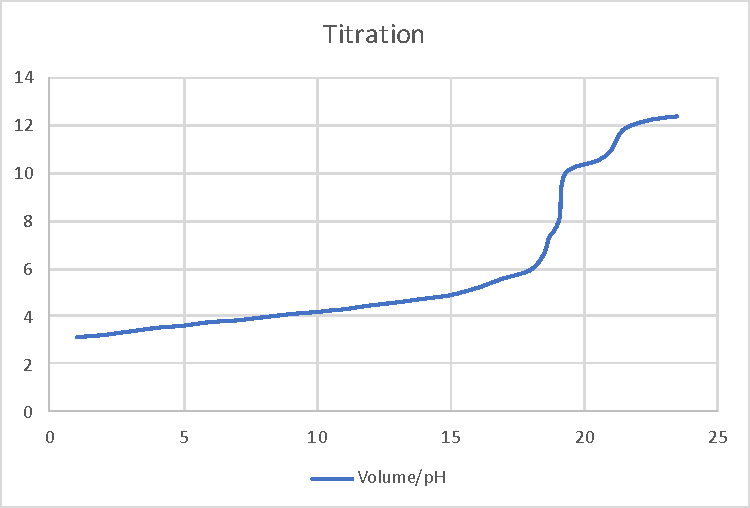
\includegraphics[scale = 0.45]{Graph.pdf}
        \caption{A graph of a Titration curve based of of data that was provided by Professor Moulds. The Volume and pH seem linear up until around 18mL where pH seems to not increase as much.}
        \label{titration}
    \end{figure}
\end{center}



\section{Mathematical formulas}
There are two ways to express formulas in \LaTeX\ . In-line and display.  In-line isplay is where your formulas show within a sentence such as \( f(x) = \sum_{i=0}^{n} \frac{a_i}{1+x} \) and this can be done by adding \textbackslash{displaystyle} in front of the mathematical expression of your choice. The other option is regular display and this method has its own section away from the sentence like so:
\begin{equation}
     f(x) = \sum_{i=0}^{n} \frac{a_i}{1+x} 
\end{equation}


It is very simple to get any mathematical symbol. All you have to do is add a \textbackslash, followed by the name of the symbol you want. But be careful, you must be in math mode or else you will get an error. For example if you wanted $\theta$ all you need to type is \$\textbackslash{theta\$} \par
Fractions are just as easy to use. In order to work with fractions, you must be in mathmode and use the command \textbackslash{frac\{\}\{\}}. Here is an example of a fraction that would produce one quarter. \textbackslash{frac\{1\}\{4\}}
\begin{center}
\begin{equation}
     \frac{1}{4}
\end{equation}
\end{center} \par
Once again, in order to work with superscripts and subscripts, you have to be in mathmode. The command to work with a superscript is written \$x \^\ \{3\}\$ and gives us $x^{3}$. While the command for a subscript \$x \_\ \{3\}\$ gives us $x_{3}$. 
\begin{center}
    \^\ for a superscript \\
    \_\ for a subscript 
\end{center}



\section{How to: Acknowledgements}
Acknowledgements are used to thank all those who helped make your document possible.



\section{How to: References}
\LaTeX\ supports bibliographies out of the box, either embedding the references in your document or storing them in an external file. It is much more convenient to use a .bib file but for the sake of the assignment we will be focusing on thebibliography environment. Here is an example below so lets break it down

\begin{thebibliography}{9}
\bibitem{latexcompanion} 
Michel Goossens, Frank Mittelbach, and Alexander Samarin. 
\textit{The \LaTeX\ Companion}. 
Addison-Wesley, Reading, Massachusetts, 1993.

\bibitem{einstein} 
Albert Einstein. 
\textit{Zur Elektrodynamik bewegter K{\"o}rper}. (German) 
[\textit{On the electrodynamics of moving bodies}]. 
Annalen der Physik, 322(10):891–921, 1905.

\bibitem{knuthwebsite} 
Knuth: Computers and Typesetting,\\\texttt{http://www-cs-faculty.stanford.edu/\~{}uno/ \\abcde.html}
\end{thebibliography} 

You must begin with a \textbackslash{begin\{thebibliography\}\{x\}} where x is the number of entries you will have in your bibliography environment ending with \textbackslash{end\{thebibliography\}} Warning, you can have a maximum of 99 items in your bibliography. \par
Within that environment you insert \textbackslash{bibitem\{id\}} where id is the identifier for that specific bibliography item. Each item typically starts with the name of the author followed by the title and where you got your information from in italics. Italics can be made using the \textbackslash{textit\{content\}} command. \par

\begin{center}
\textbackslash{label\{marker\}} : used to give the object you want to reference a marker\\
\textbackslash{ref\{marker\}} : used to reference an object with the specified marker. \\
\textbackslash{pageref\{marker\}} : used to print the page number where the object with the specified marker is found.\\ 
The following code will create two sections, one with a label and one referencing that label followed by the page it was referenced on: \\ \textbackslash{section\{Greetings\}} \\
\textbackslash{label\{sec:greetings\}} \\
Hello!\\
\textbackslash{section\{Referencing\}} \\
I greeted in section \~\ \textbackslash{ref\{sec:greetings\}} \\
I greeted in section \~\ \textbackslash{pageref\{sec:greetings\}}


\section{Greetings}
\label{sec:greetings}
Hello!
\section{Referencing}
I greeted in section~\ref{sec:greetings}.\\
I greeted on page ~\pageref{sec:greetings} \\

\textbackslash{cite\{id\}} : used to print a number of text, depending on the bibliography style, to reference the bibliography entry whose label is passed to the command 
\end{center}
You can now embed your work with citations using the command \textbackslash{cite\{id\}}, where id is the identifier you chose for each citation. If I wanted to reference Albert Einstein's \textit{On the electrodynamics of moving bodies}. I would call \textbackslash{cite\{einstein\}} and get \cite{einstein}. 

\section{Conclusion}
I hope that this tutorial finds you well and assists you in your journey with \LaTeX\ . \LaTeX\ is a fairly simple language to learn and has many uses for almost all pieces of literature. It is a very flexible tool that can turn any piece of writing into a clean masterpiece.

\section{Acknowledgements}
The research included in this document could not have been performed if not for the assistance, patience, and support of many individuals.  I would like to extend my gratitude first and foremost to my Teacher Assistant Kevin Bowden for mentoring me over the course of 4 weeks.  His insight lead me to push through this seemingly never ending assignment. The feedback from my peers, has helped me through extremely difficult times over the course of the rough draft until now. Couldn't have done it without everyone's support. Also shout out to Professor Moulds for being generous enough to give us a zip file containing a .tex file already!


\begin{thebibliography}{9}
\bibitem{item1} 
Klaus Hoppner,
\textit{Typsetting Tables with \LaTeX}. 

\bibitem{item2} 
Projects, Contributors to Wikimedia,
\\\texttt{https://en.wikibooks.org/wiki/LaTeX
/Labels_and_Cross-referencing},
Wikimedia Foundation, \\
Inc, Apr 2020

\bibitem{item3} 
Overleaf, online latex editor \\\texttt{https://www.overleaf.com/learn/latex/
Main_Page}

\bibitem{item4} 
 William L. Hosch, 
 \\\texttt{https://www.britannica.com/technology/\\LaTeX-computer
 -programming-language}

\end{thebibliography}

 



%----- Additional Features -----------------------------------------------------------------------





% You can push biographies down or up by placing
% a \vfill before or after them. The appropriate
% use of \vfill depends on what kind of text is
% on the last page and whether or not the columns
% are being equalized.

%\vfill

% Can be used to pull up biographies so that the bottom of the last one
% is flush with the other column.
%\enlargethispage{-5in}

\end{document}
